\chapter{A Large Ion Collider Experiment at the Large Hadron Collider} \label{ch:ALICE}

\section{The Large Hadron Collider}

The Large Hadron Collider (LHC) is a 27 km circumference circular hadron collider located at CERN in Geneva, Switzerland and extending into France roughly 100 meters underground. While it was originally designed to collide protons at energies of $\sqrt{s}$=13 TeV and lead ions at $\sqrt{s_{NN}}$=2.56 TeV per nucleon pair, it has since increased its collision energies for the second run. In Run 2, the LHC collided proton beams at a center-of-mass energy of $\sqrt{s}$=26 TeV and lead ions at $\sqrt{s_{NN}}$=5.02 TeV per nucleon pair. There was an additional period during which the proton beams were collided at $\sqrt{s}$=10.04 TeV for direct comparisons at the lead ion collision energy. The LHC was primarily built to discover the Higgs Boson and search for evidence of supersymmetry, but many other measurements are possible at the LHC.

The  LHC was constructed from 1998 to 2008 and began  operation in 2009. There are four major experiments situated along the ring at various interaction points: A Large Ion Collider Experiment (ALICE), A Toroidal LHC Apparatus (ATLAS), Compact Muon Solenoid (CMS), and Large Hadron Collider beauty(LHCb). A schematic of the LHC is shown in Fig~\ref{fig:LHCSchematic}. In 2012, ATLAS and CMS independently discovered the Higgs boson, marking a huge success for the LHC and the Standard Model. A majority of the effort at the LHC is devoted to increasing the integrated proton luminosity to better understand the Higgs and other rare processes. Additionally, for approximately one month out of the year, the LHC shifts focus to heavy ion collision and other systems that support heavy ion measurements. In addition to Pb- and Xe-A collisions, the periods have included smaller systems like p-Pb and pp at comparable energies to the Pb ion collisions.

\begin{figure}
    \centering
    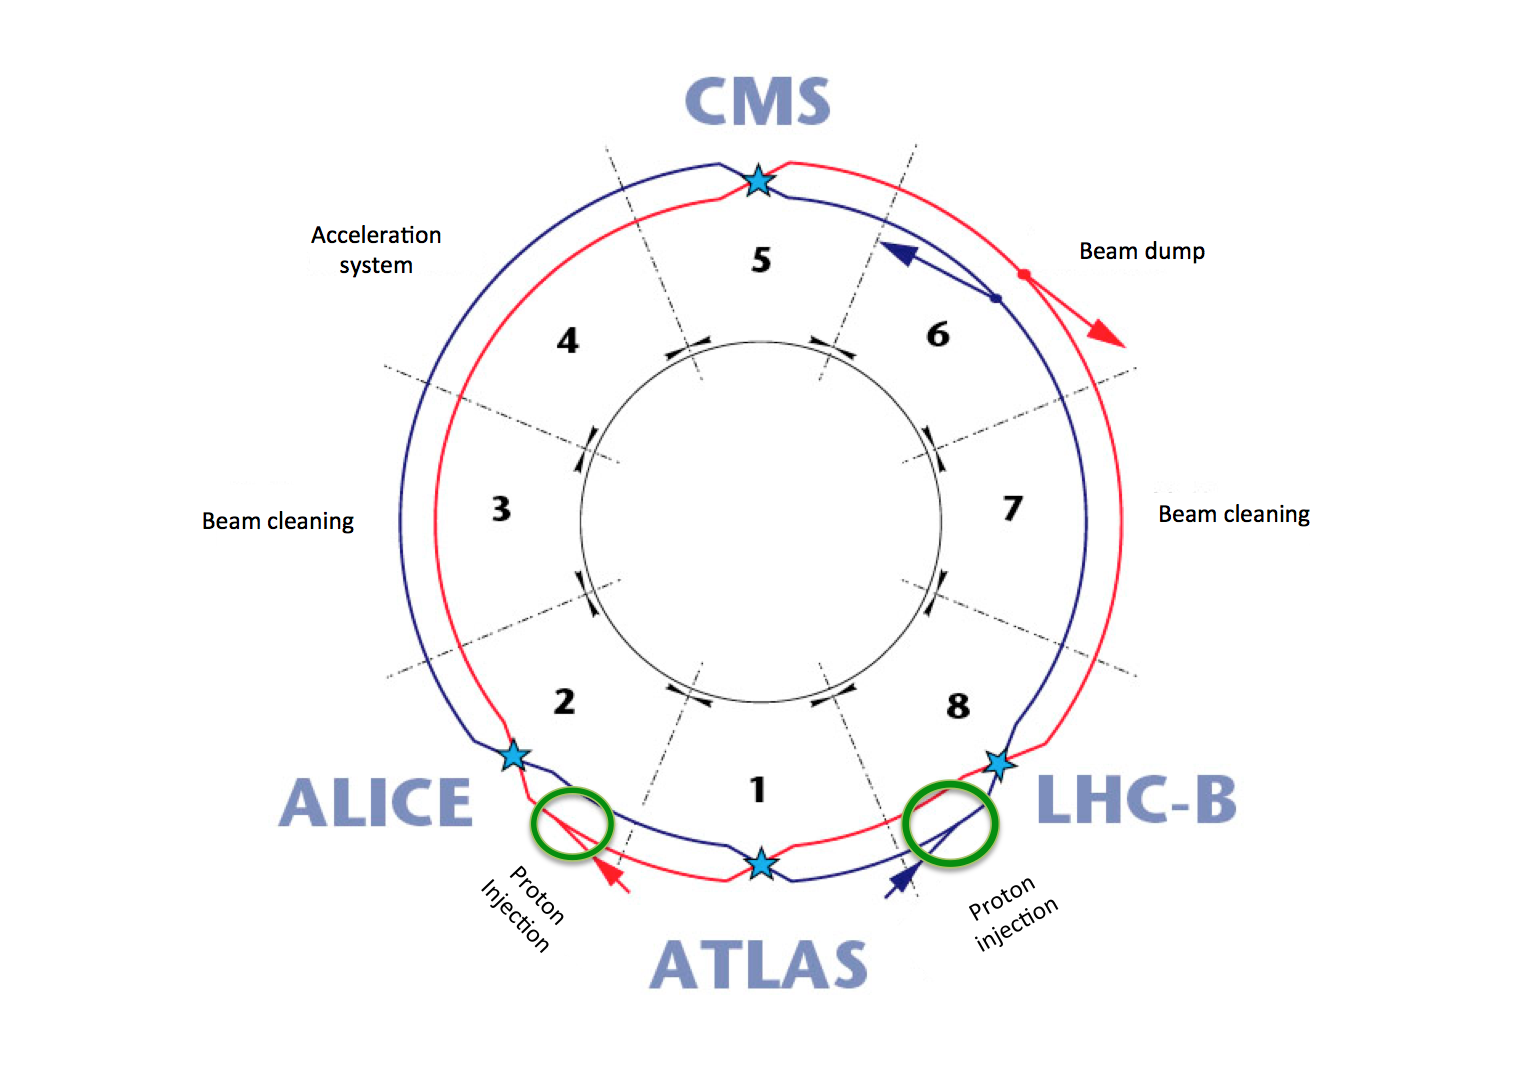
\includegraphics[width=\textwidth]{figures/png/LHC Schematic.png}
    \caption{Schematic of the LHC showing the four major experiments}\label{fig:LHCSchematic}
\end{figure}

\begin{figure}
    \centering
    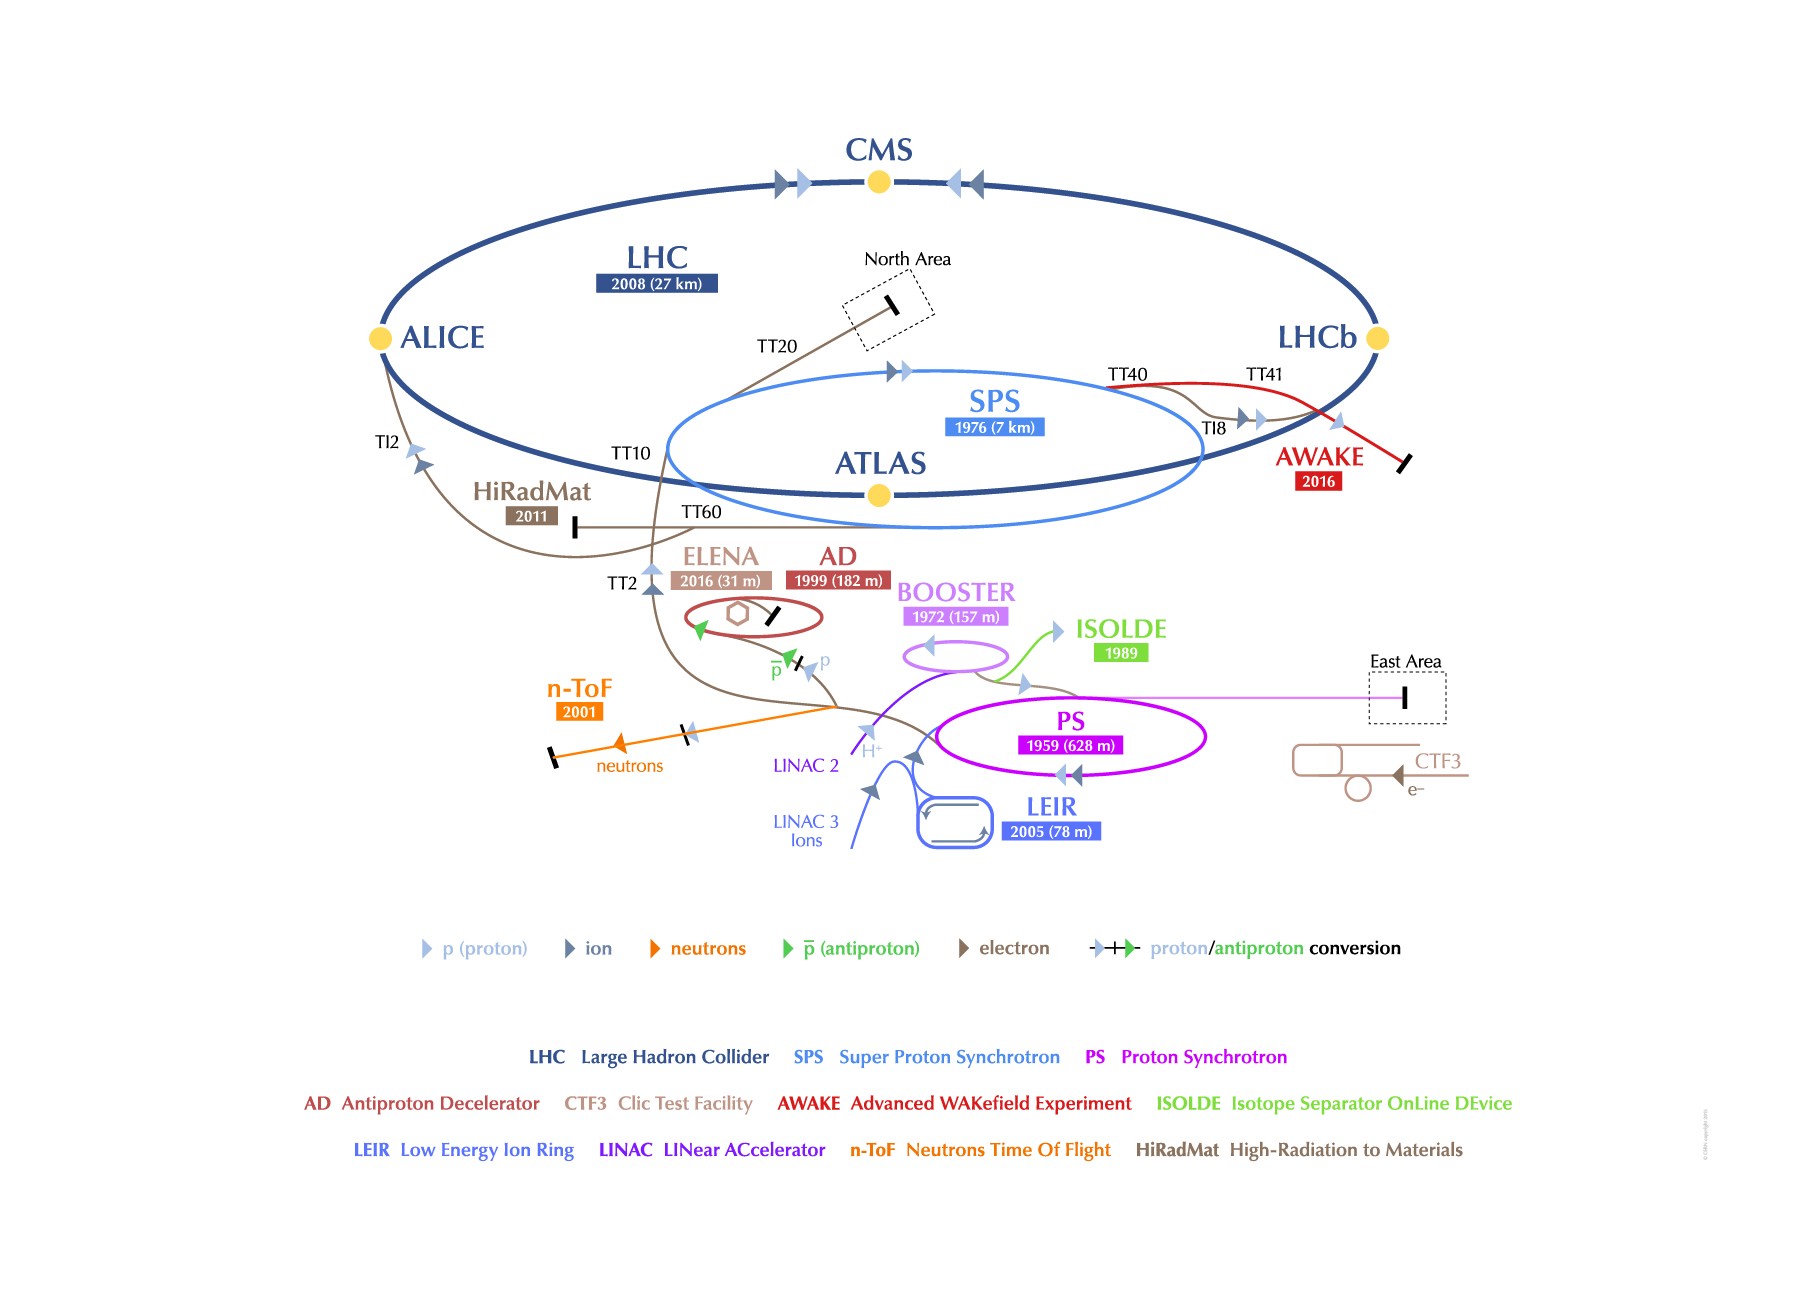
\includegraphics[width=\textwidth]{figures/png/CERN Accelerator Complex.jpg}
    \caption{CERN Accelerator Complex showing the journey that protons take to
    arrive in the LHC~\cite{CERNComplex}}\label{fig:CERNComplex}
\end{figure}

The CERN accelerator complex is shown in Figure~\ref{fig:CERNComplex}. The protons that end up in the LHC are accelerated in a series of small steps to increasingly large energies. Hydrogen gas is pumped into the Duoplasmatron Proton Source which ionizes the gas and accelerates the resulting protons to a final speed of \~1.4\% of the speed of light. After a brief trip through a radio frequency quadrupole, which further accelerates and focuses the beam, the protons are sent through the LINAC2. The protons leave the LINAC2 with an energy of 50 MeV and a mass which is 5\% higher than their rest mass. The next step is the first circular accelerator, the Proton Synchrotron Booster, which accelerates the relatively slow 50 MeV protons up to 1.4 GeV for injection into the Proton Synchrotron. Previous iterations of the proton supply chain had injected directly from the LINAC2 to the PS, but the low energy limited the intensity. Once injected into the PS, CERN's first synchrotron, the protons are accelerated to 25 GeV before entering the Super Proton Synchrotron which accelerates them to 450 GeV in preparation for the LHC. The LHC accelerates two beams of protons each to their final energy heading in opposite directions towards their final destination; one of four collision points: ATLAS, CMS, LHCb, and ALICE shown in Figure 2.2. When the LHC collides lead ions, they originate from a highly purified lead sample heated to 800 $\cdot$C. The resulting lead vapor is then ionized and is transported through the LINAC3 to the LEIR. From there, the ions are transported via the same acceleration chain as protons. Optimizing the details of every step in the acceleration chain and maintaining the beams within the LHC is a complicated task that requires monitoring and adaptive action. The measurements that we do would not be possible without the diligent efforts of the LHC operations staff.



\section{A Large Ion Collider Experiment}
The ALICE detector is specifically designed to analyze the products of heavy-ion collisions in the LHC. The ALICE detector is shown in Figure~\ref{ALICEDetector}. The total volume of the detector is 16 x 16 x 26 $m^3$. The total weight of the ALICE detector is approximately 9000 metric tons. Surrounding the entire experiment is the L3 solenoid magnet which serves to bend the tracks for momentum measurements using a field of 0.50 T. The ALICE detector is composed of several sub-detectors which provide specific functionality. The main tasks of the ALICE detector are triggering, tracking, particle identification, and calorimetry. Triggering signals when an interesting event is occuring so that it can be written out to disk. Tracking provides position and momentum information through a large volume of the detector. Particle identification(PID) leverages many sub-detectors to identify particle species. Calorimetry provides a direct measurement of the energy.

Triggering uses information processed in the Central Trigger Processor from several sub-detectors to make the decision to write the event to disk or not. The sub-detectors which provide triggers include the V0, T0, and the EMCal. Tracking encompasses the group of sub-detectors in the Central Barrel; these include the ITS and the TPC. Coupled with the L3 magnet, we can provide positional tracking in the central barrel and momentum information for charged particles. Several detectors in ALICE provide signals that are used for particle identification. The ITS and TPC provide energy loss vs. momentum measurements, and the TOF provides time-of-flight measurements. The TRD allows discrimination based on transition radiation behavior, and the HMPID extends the identification capabilities for p and K to higher momentum via ring-imaging Cherenkov detectors. Calorimetry is composed of three electromagnetic calorimeters: the EMCal, DCal, and the PHOS.The EMCal and DCal are situated roughly 180$\cdot$ in $\phi$ from each other allowing for dijet measurements, and the PHOS is a very high resolution calorimeter used primarily for photon measurements. The following sections will describe the sub-detectors which are used in my analysis in more detail.

\subsection*{V0 Detector}

The V0 detector is a two-layered array of 32 scintillation counters. It is installed around the ALICE interaction point in two pieces, V0A and V0C, covering the backward and forward regions, respectively. The V0 detector's main functions are providing Minimum Bias and Centrality triggers, measuring the reaction plane resolution, and determining the centrality for p-p and A-A collisions. The detector covers pseudorapidity ranges 2.8 < $\eta$ < 5.1 (V0A) and -3.7 < $\eta$ < -1.7 (V0C) with full azimuthal coverage. The V0A array is located 330 cm in front of the IP along the beam line on the A side, the V0C array is located 90 cm after the IP along the beam line. Each array is segmented into counters separated into four ring structures. This is shown below in Figure~\ref*{fig:V0Detector}.

The Minimum Bias trigger requires signal in both arrays for an event to be recorded; this is referred to as AND mode. In addition, one can require more specific triggers: Multiplicity Trigger, Semi-Central trigger, Central Trigger, and a Minimum Bias p-Gas trigger. In realistic p-p collisions, for non-diffractive collisions, the V0 will detect at least one charged particle in both arrays with an efficiency of approximately 84\%. In this analysis we use the Minimum Bias trigger to select events in p-p collisions and both the Central and Semi-Central triggers to select events in Pb-Pb collisions.

The V0 detector provides a measurement of the charged particle multiplicity based on the energy deposited in the scintillators. A detailed simulation of the V0 apparatus was used to extract the relationship between charge collected inside a V0 ring and the charged particle multiplicity in the corresponding $\eta$ range. The distribution of charged particle multiplicities, $\frac{dN_{ch}}{d\eta}$ is then obtained in $\eta$ bins corresponding to the scintillator rings of the V0. Figure~\ref{fig:V0Amplitudes} shows an example of a distribution of V0 amplitudes. This distribution is fit using a Monte Carlo Glauber model which reproduces the V0 amplitude distribution, and hence the centrality, for all but the most peripheral collisions. For low multiplicity events, the most peripheral collisions, the minimum bias trigger efficiency is not 100\%, therefore we extrapolate the Glauber fit to the most peripheral centralities.

The V0 detector additonally provides an measurement of the event plane, $\Psi_n$, an experimental determination of the true reaction plane, $\Psi_{RP}$ . The event plane is used in the analysis of anisotropic particle flow, a central component of the Reaction Plane Fit background subtraction method used in this analysis. The determination of the event plane is described in~\ref{sec:EP_determination} along with a discussion of the corrections. The V0 detector is also used to determine the reaction plane resolution, the accuracy with which the event plane reproduces the true orientation of the reaction plane. This is described in [20]. The reaction plane resolution depends on the multiplicity of charged particles in the collision. This is shown in Figure~\ref{fig:RPResolution}.

\subsection*{T0 Detector}

The (T0) detector consists of two arrays of Cherenkov counters, T0C and T0A on either side of the interaction point. The T0 detector is used to provide a start time for the Time-of-Flight detector, described in~\ref{subsec:TOF}. The T0 detector is also used to measure the vertext position as a backup of the V0 functionality. Each detector array is composed of 12 cylindrical counters coupled with photomultiplier tubes. The T0C and T0A arrays are located at approximately 70 cm and 370 cm away from the interaction point respectively. They both cover the full range of azimuth as well as -3.28 < $\eta$ < -2.97 (T0C) and 4.61 < $\eta$ < 4.92 (T0A). Figure~\ref{fig:T0InteractionTime} shows the interaction time measured in the T0 with respect to the LHC clock, and Figure~\ref{fig:T0Resolution} the resolution measured as the difference between the T0A and T0C.The T0 detector is used in this analysis to provide a start time for the TOF detector.

\subsection*{Inner Tracking System}

The Inner Tracking System (ITS) detector is composed of six concentric layers of cylindrical silicon detectors: two layers each of the Silicon Strip Detector (SSD), Silicon Drift Detector (SDD), and Silicon Pixel Detector (SPD). The ITS has the main functions of measuring primary and secondary vertices, as well as augmenting the barrel tracking and particle identification capabilities. The ITS surrounds the interaction point with a full azimuthal range, psuedorapidity |$\eta$| <0.9, and a radial coverage of 3.9cm < r < 43.0cm. The SDD and SSD both provide a read-out of the signal amplitude and thus contribute to PID in ALICE through $\dEdx$ measurements. Using a truncated mean of up to four signals we measure a $\dEdx$ resolution of 12\%~\cite{}. Figure~\ref{fig:ITSSchematic} shows a schematic view of the ITS with the SPD, SDD, and SSD layers highlighted in stereographic (left) and transverse (right) projections.

We do not use the ITS for particle identification in this analysis. This is because the momentum range in which the ITS can effectively separate particle species is below 1 GeV/c and this analysis does not consider these particles. Figure~\ref{fig:ITSEnergyLoss} shows the energy loss of hadrons traversing the ITS as a function of momentum.

\subsection*{Time Projection Chamber}\label{subsec:TPC}

The ALICE Time Projection Chamber is a 92 $m^3$ cylindrical barrel filled with a gas mixture of 10\% CO2 and 90\% Ne. The barrel has a radial extent of 84.8 cm < r < 246.6cm, covering the full azimuth and |$\eta$| < 0.9. It is separated by its axial center into two drift regions which comprise the primary tracking volumes in ALICE, shown in Figure 2.10. The TPC provides tracking for charged particles moving through its active volume. Charged particles traverse the drift regions and ionize gas along their path. The drift regions provide a constant drift field along the beam direction of 400 V/cm that directs the liberated electrons towards the anodes located at the end caps of the TPC. The electrons induce an avalanche effect on the wires near the anode providing the necessary signal amplification for readout. The TPC contains 557568 readout channels and has a resolution of 800 to 1100 $\mu$m in the R and $\phi$ directions, and 1100 to 1250 $\mu$m in the direction of the beam axis. 

Particle identification can be done in the TPC for pions, protons, kaons and
electrons by measuring the specific energy loss, $\dEdx$, due to ionization as these particles
traverse the gaseous volume. The $\dEdx$ measurements for the TPC are shown for p-p collisions at 7 TeV in Figure~\ref{fig:TPCdEdx}. The specific energy loss is calculated using the Bethe-Bloch formula, however, experimentally other parametrizations are used which simplify calculations for specific gas mixtures. The solid lines in Figure~\ref{fig:TPCdEdx} are given by the ALEPH parameterization of the Bethe-Bloch fromula given in Eq~\ref{eq:TPCdEdx}. The parameters are fixed by the gas mixture. The TPC has an average $\dEdx$ resolution of $\sigma(\dEdx)/\left<\dEdx\right>$ = 7\%, but in general the resolution scales inversely with the square root of the number of TPC track points for the track in question, $\sigma(\dEdx)$ $\propto$ 1/$\sqrt{n}$.

\begin{equation}\label{eq:TPCdEdx}
    f(\beta \gamma) = \frac{P_1}{\beta^{P_4}}\left(P_2 - \beta^{P_4} - \ln \left(P_3 + \frac{1}{(\beta \gamma)^{P_5}}\right)\right)
\end{equation}

The TPC can be used to identify particle species on a track-by-track basis at low momentum, and statistically at higher momentum. In this analysis we apply the statistical technique described in~\ref{subsec:PID} across the entire momentum range. 

\subsection*{Electromagnatic Calorimeter}\label{subsec:EMCal}

The ALICE Electromagnetic Calorimeter and Dijet Calorimeter are lead scintillating detectors designed to measure the electrons from heavy-flavor hadron decays,the electromagnetic component of jets, and spectra of direct photons and neutral mesons. The calorimeters enable triggering and full reconstruction for jets within their acceptances. The EMCAL covers a range of 107 $\cdot$ in $\phi$ and |$\eta$| $\leq$ 0.7, and the DCAL in $\phi$ and |$\eta$| $\leq$ 1.4. The EMCAL is segmented into 12288 6.0 cm x 6.0 cm x 24.6 cm optically isolated rectangular prisms (towers) of 76 alternating layers of the scintillator (Polystyrene) and absorber (Pb). The towers are grouped into units called supermodules. The DCAL is constructed from the same technology used in the EMCAL. Figure~\ref{fig:EMCalSM} shows a drawing of one of the super modules.

When a particle is incident on the calorimeter, the particle’s energy is deposited in the detector, producing light via scintillation. Scintillation is the process where a material will re-emit energy absorbed as light when struck with ionizing radiation. The light then travels through fiber optic cables terminating at avalanche photo- diodes. The resulting amplified signal is fed into a charge sensitive pre-amplifier and digitized using the Front End Electronics cards.

The EMCal can be used for a high-purity identification of electrons due to the fact that they deposit almost all of their energy in the EMCal. Figure~\ref{fig:EMCalEoverP} shows the ratio of the energy measured in the EMCal detector to the momentum measured in the TPC for a given particle. Only electrons deposit most of their energy in the EMCal resulting in a peak near one, hadrons typically do not deposit all of their energy within the radial length of the EMCal.

The calorimeters are used in order to trigger on jet events as well as to study the neutral component of jets. They are designed with triggering electronics for a fast, efficient high-pT jet trigger. With an enhanced sample of events containing high-pT jets, we can study jets with lower uncertainty. Furthermore, measuring the neutral component of jets allows us to study the full energy content of jets. This allows us to compare jet measurements to perturbative calculations directly. In this analysis we do not use the jet trigger so as to avoid any potential bias in the jet spectrum. We use the calorimeters to measure the neutral component of jets. This is described in~ref{sec:Jets}.

\subsection*{Time-of-Flight Detector}\label{subsec:TOF}

The ALICE Time-of-Flight (TOF) Detector is a large area array of Multi-gap Resistive Plate Chambers (MRPCs) designed to provide particle identification for charged particles in the intermediate momentum range. Additionally, the TOF serves as a trigger for cosmic and ultra-peripheral events. The TOF covers a range of |$\eta$| < 0.9 and 2$\pi$ in $\phi$. The TOF is composed of 1593 MRPC strips arranged in 18 azimuthal sectors. On average, the TOF provides a time resolution of 80 ps.

The TOF provides PID for charged particles by comparing the measured time-of-flight of each track with the expected time-of-flight for a given particle species at a given momentum. Figure~\ref{fig:TOFPID} shows the particle velocity ($\beta$ = v/c) as a function of momentum. The pion, kaon, and proton bands are labeled along with electrons and deuterium. The TOF provides clean separation between pions and kaons up to momentums of roughly 3 GeV/c and clean separation between protons and kaons up to momentums of roughly 5 GeV/c. The TOF is used in this analysis to provide clean samples of pions, kaons and protons for further analysis. This is described in~\ref{sec:PID}. 

